\documentclass[10pt]{article}
%\usepackage{widetext}
\usepackage{cite}
\usepackage{amsmath}
\usepackage{enumerate}
\usepackage{array}
\usepackage{subfig}
\usepackage{graphicx}
\usepackage{float}
%\usepackage[footnotesize,bf]{caption}
%\usepackage{subcaption}
\usepackage{amsfonts}
\usepackage{amssymb}
\usepackage{epstopdf}
\usepackage[cm]{fullpage}
\usepackage{multicol}
\usepackage{multirow}
\usepackage{authblk}
\usepackage{mathtools}
\usepackage{titlesec}
\usepackage{booktabs}
\usepackage{xr}
\externaldocument{Supplement}


%\usepackage{ amssymb }

\setlength{\parskip}{0ex plus0ex minus0ex}
%\setlength\parindent{10pt}
\setlength{\columnsep}{1cm}

\titleformat{\section}
  {\normalfont\sffamily\Large}
  {\thesection}{0.5em}{}
  
\titleformat{\subsection}
  {\normalfont\sffamily\large}
  {\thesubsection}{0.5em}{}

\titleformat{\subsubsection}
  {\normalfont\sffamily\normalsize}
  {\thesubsubsection}{0.5em}{}

\titlespacing*\section{0pt}{20pt plus 4pt minus 2pt}{5pt plus 2pt minus 2pt}
\titlespacing*\subsection{0pt}{16pt plus 4pt minus 2pt}{4pt plus 1pt minus 1pt}
\titlespacing*\subsubsection{0pt}{12pt plus 4pt minus 2pt}{2pt plus 0pt minus 0pt}




\title{\vspace{-1.5cm}\sffamily Social fluidity mobilizes infectious disease in human and animal populations}
\date{}
\author[1]{Ewan Colman\footnote{ec975@georgetown.edu}}
\affil{\small{Department of Biology, Georgetown University, Washington, DC 20057, U.S.A}}
%\author[2]{Andreas Modlmeier}
%\author[2]{David Hughes}
%\affil{\small{Departments of Entomology and Biology, Penn State University, PA 16802, U.S.A}}
\author[1]{Shweta Bansal}
\renewcommand\Authands{ and }
\begin{document}
\maketitle
\vspace{-0.7cm}
\begin{abstract}
\noindent\normalsize
This paper introduces a novel method to quantify sociality in human and animal populations and explores the connection between social behaviour and the spread of infectious disease. Individuals living in groups tend to distribute their social effort heterogeneously, with some group members receiving more attention than others. By incorporating this heterogeneity into a mathematical model, we find that a single parameter, which we name Social Fluidity, controls the level of social mixing in the population. We estimate the social fluidity of $51$ empirical human and animal social systems using maximum likelihood techniques. An analytical formula that connects social fluidity to both the population size and the basic reproductive number of an infectious disease is derived and simulations of the spread of disease are performed. We find that social fluidity outperforms other network-based metrics in predicting the basic reproductive number of an infectious disease and that the effect of population size on disease transmission is insignificant compared to the effect of social fluidity.
\end{abstract}
\vspace{0.5cm}
\begin{multicols}{2}

%%%%%%%%%%%%FIGURES%%%%%%%%%%%%%%%%%%%%%%%%%%%%%%%%%%%%%%%%%%%%%%%%%%%%%%%%%
\begin{figure*}[t]
	\centering
	\includegraphics[width=0.8\textwidth]{Figures/concept_fig.png}\qquad	
  	\caption{\textbf{Left:} Each individual can be represented as a single point on this plot. Dashed lines mark the boundary of the region where data points can feasibly be found. The thick black lines represent two possible types of social behavior; as the number of observed interactions grows, the set of social contacts increases; the rate at which it increases influences how we categorize their social behaviour. \textbf{Middle:} The width of the lines between $i$ and the other circles represents the propensity of $i$ to interact with each of the other members of the population. \textbf{Right:} Probability distributions that correspond to the different levels of heterogeneity in the contact propensities, both distributions are expressed by Eq.\eqref{distribution}.\label{concept_fig}}
\end{figure*}

\begin{figure*}[t]
	\centering
	\includegraphics[width=0.6\textwidth]{Figures/interaction_types.png}
  	\caption{\textbf{A:} Each point represents a human or animal system for which social fluidity was estimated. Vertical lines show the standard error of the estimate. The systems are organized according to the type of interaction that was recorded: aggression includes fighting and displays of dominance, food sharing refers to mouth-to-mouth passing of food, antennation is when an insects antenna touches any part of another individual, territorial interaction refers to animals that come close to each other during foraging, face-to-face refers to close proximity interactions between people, association is defined as co-membership of the same group same group. These results are also presented in Table \ref{results_table} of the online supplement. \label{phi_for_all_networks}}
	\label{phi_fig}
\end{figure*}

\begin{figure*}[t]
 \centering
 \includegraphics[width=\textwidth]{Figures/disease_theory.png}
\caption{\textbf{A:} Each point represents a human or animal data-set. For each one, $R_{0}$ is calculated from Eq.\eqref{R_0_solution} for every individual in the population and the mean ($\pm$ one standard error) is plotted against its corresponding value of $\phi$. These results are also presented in Table \ref{results_table} of the online supplement. \textbf{B:} Theoretical results from Eq.\eqref{R_0_solution}; the relationship between $R_{0}$ and population size is shown to depend on the value of $\phi$. \textbf{C:} In large populations $R_{0}$ increases with $\phi$ up to $\phi=1$. \label{disease_theory}}
\end{figure*}

\begin{figure*}[t]
	\centering
	\includegraphics[width=\textwidth]{Figures/R0_for_all_networks.png}\qquad	
  	\caption{Each point represents a human or animal data-set for which the time of interactions appear in the data. For each one, $R_{0}$ for every individual in the population is found by simulating disease spread and the mean ($\pm$ one standard error in \textbf{A}) is plotted against its corresponding value of $\phi$ and other population metrics. These results are also presented in Table \ref{results_table} of the online supplement.\label{disease_simulation_fig}}
\end{figure*}
%%%%%%%%%%%%%%%%%%%%%%%%%%%%%%%%%%%%%%%%%%%%%%%%%%%%%%%%%%%%%%%%%%%%%%%%%%%%%%%%%%%%%%

\section{Background}
%\label{background}
Socialization is fundamental to the well-being of humans and the survival and many animal species \cite{Brent20170515,10.1371/journal.pmed.1000316,silk2007adaptive}. To receive the fitness benefits of group membership, individuals must engage in social activities such as grooming, food-sharing, and conversation, in order to maintain a healthy and stable society \cite{SUEUR2011156,krause2002living}. In addition to many factors including time, energy, resource availability, and cognition \cite{kappeler2013constraints,LEHMANN20071617}, it is commonly thought that the threat of infectious disease imposes a limit on the social capacity of animal groups \cite{freeland1976pathogens, altizer2003social}.

Larger populations are assumed to provide a greater number of opportunities for an infectious disease to transmit. For this to be true, however, the number of potential pathways for disease transmission must scale accordingly \cite{de1995does,ferrari2011pathogens}. Moreover, some empirical results contradict the hypothesis that disease risk increases with group size \cite{rifkin2012animals,patterson2013parasite}. Since the contact structure of the host population and the mode of transmission both play a role, the relationship between group size and epidemic risk is complex \cite{Smith12052009,ECY:ECY20139492076,borremans2016nonlinear,HOCK201234,Sah18042017}.

Networks provide some understanding towards the role of within-group contact structure \cite{doi:10.1093/beheco/art047}. It is recognized that the degree of an individual in a social network, i.e. the number of other individuals with whom they interact, has epidemiological significance \cite{Bansal879}. While an increase in population size may cause an increase in the degree of an individual, some of these ties may weaken as a result. In humans, for example, social effort is invested mostly in close friends and family members, less is invested in the wider friendship circle, and as the circle extends to a wider group of people the frequency of interaction decreases \cite{MacCarron2016151,saramaki2014persistence,10.1371/journal.pone.0022656}. 

It has been proposed that a better understanding of this aspect of social behaviour may lead to a quantitative approach to comparing sociality across species \cite{dunbar2010bondedness}. We further suggest that it will lead to better understanding of disease spread \cite{karsai2014time}. While there is a significant epidemiology literature that challenges the assumption of homogeneous mixing \cite{anderson1992infectious, castillo1989epidemiological, DelValle2007539, Volz2925}, no effort has previously been made to quantify the level mixing in a way that allows comparison across a range of animal disease systems. 

In this paper we develop a mathematical model of human and animal social behaviour in which one parameter controls the heterogeneity in the way individuals choose to distribute their social effort. In the context of disease transmission, the same parameter, which we call ``social fluidity'' can be interpreted as the amount of mixing within the population. By estimating the social fluidity in a number of human and animal social systems we find evidence that opposes the hypothesis that the threat of infectious disease imposes limitations on group size.  

\section{Methods}
\subsection{Social behavior model}
\label{social_behavior}
Our analysis concerns a closed system of $N$ individuals and a process of interaction that may occur between pairs of individuals. The system can be thought of as a network; an individual human or animal, which we call $i$, is a node; the weight $w_{i,j}$ is the number of times two nodes $i$ and $j$ were observed interacting together; if $w_{i,j}>0$ then we say that an edge exists between $i$ and $j$; the number of times that $i$ was observed interacting is its strength, $s_{i}$ ($s_{i}=\sum_{j}w_{i,j}$); and the number of partners with whom $i$ was observed interacting is its degree, $d_{i}$. 

We consider the interactions of one node, $i$, which we call the focal node. The relationship between $s_{i}$ and $d_{i}$ is analogous to the relationship between the number of animals observed and the number of species observed in wildlife surveys \cite{hurlbert1971nonconcept, burnham1978estimation, colwell2004interpolating}. Just as each new animal observation can either return a previously unobserved species or one that has been observed before, each observed interaction of $i$ can either return a new interaction partner or one that $i$ has interacted with before. The likelihood of sampling a given species, in this case, is replaced with a the likelihood that $i$ will interact with $j$, where $j$ is any other member of the population. Formally, we define $x_{j|i}$ to be the probability that $j$ is the interaction partner of $i$ given that $i$ is observed in an interaction. 

Applying a similar approach to early work in species accumulation curves \cite{arrhenius1921species}, the probability that $i$ has interacted with $j$ at least once over the course of $s_{i}$ observations is
\begin{equation}
\label{i_to_j}
P(i \rightarrow j|s_{i})=1-(1-x_{j|i})^{s_{i}}.
\end{equation}
In our model we assume that the values of $x_{j|i}$ over all $i,j$ pairs are distributed heterogeneously according to a probability distribution, $\rho(x)$. Thus, the probability that an edge exists between any chosen focal individual $i$, and any given member of the population is no longer specific to the particular choice of $i$ and $j$. The general formula for the probability that an edge exists between the focal individual and any other individual in the population, after $s$ observations, is 
\begin{equation}
\label{i_to_any}
\Psi(s)=1-\int\rho(x)(1-x)^{s}dx.
\end{equation}

Our goal is to find a form of $\rho$ that accurately reproduces the degree distributions seen in real social systems. This can be achieved with the following truncated power law,
\begin{equation}
\label{distribution}
\rho(x)=\frac{\phi\epsilon^{\phi}}{1-\epsilon^{\phi}}x^{-(1+\phi)} \text{ for } \epsilon<x<1.
\end{equation}
The terms in this expression are explained as follows: the quotient on the left ensures that $\rho(x)$ meets the requirement of a probability density function that $\int\rho(x)dx=1$, $\epsilon$ truncates the distribution to avoid an asymptote at $x=0$, $\rho(x)$ is also truncated $1$ to ensure that all values of $x_{j|i}$, which are probabilities, are less than $1$, and finally, $\phi$ is a parameter that controls the heterogeneity in the values of $x_{j|i}$. 

While the model contains two parameters, $\epsilon$ and $\phi$, the requirement that $\sum_{j}x_{j|i}=1$ can only be met if $\epsilon=\epsilon(N,\phi)$ is chosen to be a specific value (a detailed explanation of how to compute $\epsilon$ is included in the online supplement \ref{epsilon}). Larger values of $N$ correspond to smaller values of $\epsilon$ and so larger populations see a higher frequency of weak relationships, i.e. small values of $x_{j|i}$. Since $\phi$ is the only free parameter in the model, and is therefor the only determinant of social behaviour, we use the term ``social fluidity'' to refer to this quantity.  

Figure \ref{concept_fig} illustrates how the value of $\phi$ can create different types of social behaviour. Low values of $\phi$ produce a type of social behaviour that we might describe as ``allegiant''; interactions with the same partner are frequently repeated at the expense of interactions with unfamiliar individuals. As $\phi$ increases, the model produces more ``gregarious'' behaviour; interactions are repeated less frequently and the number of partners is larger. High social fluidity corresponds to a high level of mixing withing the population or social group.

Combining Eq.\eqref{i_to_any} and Eq.\eqref{distribution} we find that, for an individual that has been observed $s$ times,
\begin{equation}
\label{hyper_solution}
\Psi(s)=1-\frac{\phi\epsilon^{\phi}(1-\epsilon)^{s+1}}{(1-\epsilon^{\phi})(s+1)}{}_{2}F_{1}(s+1, 1+\phi, s+2, 1-\epsilon)
\end{equation}
where the notation ${}_{2}F_{1}$ refers to the Gauss hypergeometric function \cite{absteg}. The probabilty that the observed degree of a node is equal to $d$ is determined by $N-1$ independent Bernoulli trials, each with success probability $\Psi(s)$. The degree distribution therefore binomial $d(s)\sim B(N-1,\Psi(s))$, however, since this distribution gives non-zero probabilities for cases where $d>s$, which are invalid, we instead use $d(s)\sim B(s,(N-1)\Psi(s)/s)$ when $0<s<N$.

We use maximum likelihood estimation to fit this model to the empirical data and return the social fluidity $\phi$ (details are contained in the online supplement \ref{fitting}). The goodness-of-fit is calculated by comparing its likelihood to the likelihood of a null model in which the degree of each individual is a uniformly distributed random integer within the range of feasible values (details are contained in the online supplement \ref{fitting}).

\subsection{Disease transmission}
\subsubsection{Analytical model}
\label{disease_section}
Our goal is to analyse how social fluidity and population size influence the likelihood of epidemic outbreaks. We do this by deriving analytically the rate of infection for a model of disease transmission in a population whose contact dynamics follow the model of the previous section. This results in a formula that predicts $R_{0}$, which is defined as the number of secondary infections caused by a single infectious individual in an otherwise fully susceptible population. We calibrate the disease parameters in a way that controls for the fact that rates of activity may vary between different populations. This results in a formula that quantifies the effect size of social fluidity that can be applied across a range of social systems. 

The disease model is described as follows: an individual becomes infectious at some random point in time and may recover at any subsequent point in time, the probability of recovery during a $1$ second interval is $\gamma$. Interactions that occur during this infectious period result in the interaction partner becoming infected with probability $\beta$. This simple disease model disregards the fact that interactions vary in duration, intimacy, and contact type (for which we often do not have data); $\beta$ here represents a probability of infection that combines all of these factors.

We first predict the reproductive number, $R_{0}(s_{i})$, of an individual who was observed interacting $s_{i}$ times during an observation period of duration $\Delta t$. The rate of activity, in this case, is estimated to be $s_{i}/\Delta t$ interactions per unit of time. By assuming that these interactions occur according to a Poisson process, transmission of the disease from the infected individual, $i$, and another individual in the population, $j$, also occurs as a Poisson process with rate $s_{i}x_{j|i}\beta/\Delta t$. The length of time for which $i$ remains infectious is exponentially distributed with rate parameter $\gamma$. For an infectious period of length $\tau$, the probability that the infection transmits from $i$ to any given $j$ is
\begin{equation}
\label{first_T}
T_{i\rightarrow j}(\tau,s_{i},x_{j|i})=1-\exp(s_{i}x_{j|i}\beta\tau/\Delta t).
\end{equation}
The reproductive number for $i$, $R_{0}(s_{i})$, is found by integrating Eq.\eqref{first_T} over all possible values of $\tau$ and $x_{j|i}$ then multiplying by the number of susceptible individuals, $N-1$. The result is given in section ... of the online supplement.

The range of human and animal systems is diverse, and social activity can happens on extremely different time-scales. Additionally, the type of diseases that affect one species is unlikely to affect another. Instead of choosing parameter values that relate to some specific disease, it is more informative to select parameter values for each system separately in a way that exposes the effects of population size and social fluidity. To achieve this, the recovery rate, $\gamma$, is chosen in such a way that $R_{0}$ would always be the same value if, hypothetically, the effects of social fluidity and population size were not present. 

We define $R^{*}$ to be the value of $R_{0}$ in a large population with homogenous mixing. Calibration is achieved when $\gamma$ is chosen to be  
\begin{equation}
\gamma=\frac{\beta\langle s\rangle}{ \Delta_{t} R^{*}}
\end{equation}
where $\Delta_{t}$ is the duration of the time-frame of the data and $\langle s\rangle$ is the mean of $s_{i}$ over the whole population. The effect of this calibration is that the recovery rate, $\gamma$, is proportional to the mean rate of activity. Consequently, a population with a higher frequencey of social interaction will be coupled with a disease that has a longer mean infectious period. 

After performing the calibration we arrive at the following result for the basic reproductive number of an individual that was observed interacting $s$ times,
\begin{equation}
\label{R_0_solution}
\begin{split}
R_{0}(s)=&\frac{1-\phi}{\phi(\epsilon^{\phi}-\epsilon)}\left[1-\epsilon^{\phi}+\epsilon^{\phi}{}_{2}F_{1}(-\phi,1,1-\phi;-R^{*}s/\langle s \rangle)\right.\\
&\left.-{}_{2}F_{1}(-\phi,1,1-\phi;-\epsilon R^{*}s/\langle s \rangle)\right].
\end{split}
\end{equation}
Note that no temporal information appears in this equation. In all the analysis presented we arbitrarily choose $R^{*}=2$. 

\subsubsection{Disease simulation}
Because the fidelity of the social behavior model, i.e. the extent to which it agrees with the data, varies across the different social settings, we expect that the accuracy of Eq.\eqref{with_N} to vary. To test this we simulated the transmission for each individual (reported results are the mean of $10^{3}$ simulations). For the simulations we arbitrarily chose a transmission probability of $\beta=1/4$ [need to justify this]. The mean absolute error $|e|$ measures the mean difference between the individual reproductive number, $r_{i}$, calculated from Eq.\eqref{with_N} and computed by the simulation. A full description of the disease simulation can be found in the online supplement. Full details are provided in Section \ref{simulation} the online supplement.

\section{Results}
\subsection{Measuring social fluidity}
Social fluidity, $\phi$, quantifies heterogeneity in the way individuals distribute their social effort among the other members of the population. We estimated $\phi$ in $51$ data-sets taken from $18$ studies of human and animal social behaviour \cite{Smith12052009, borremans2016nonlinear, 10.1371/journal.pone.0023176, 10.1371/journal.pone.0136497, 10.1371/journal.pone.0073970, Carter20122573, Grant1973449, levin2016stress, sailer1984proximity, massen2013stability, sade1972sociometrics, butovskaya1994structure, takahata1991diachronic, hass1991social, lott1979dominance, SCHEIN195545, hobson2015social, 10.1371/journal.pone.0020298}. Details of each data source are included in the online supplement \ref{data}. Figure \ref{Degree_vs_int} shows the data and the distribution fitted using maximum likelihood estimation. We find that the model provides a good fit to every data-set; model fidelity is positive in every case, which implies that the empirical data follows the model better than synthetic data generated from a mixture of $92\%$ from the model distribution and $8\%$ from random noise (see online supplement \ref{fitting}). 

Social fluidity does not appear to be affected by the sample size; there is no significant correlation between the mean number of observations per individual, $\bar{s}$, and $\phi$ (Pearson $R^{2}=0.004$, $p=0.663$). Larger populations tend to have smaller social fluidity values (Pearson $R^{2}=0.223$, $p<0.001$). This correlation is dependent on the presence of a few large populations in our data ($N>200$) which may be, to some degree, subdivided into smaller groups. As a consequence, the social effort of one individual becomes concentrated on a relatively small proportion of the whole population, which causes heterogeneity to increase, and $\phi$ to decrease.

Populations with higher values of $\phi$ tend to have higher mean degree (Pearson $R^{2}=0.332$, $p=0.001$) and less heterogeneity in the distribution of edge weights (measured as the variance divided by the mean $\sigma_{w}^{2}/\langle w\rangle$)  (Pearson $R^{2}=0.332$, $p=0.001$). Incidentally, weight heterogeneity and mean degree are uncorrelated (Pearson $R^{2}<0.001$, $p=0.984$). The fact that social fluidity correlates with both the weight heterogeneity and the mean degree, yet they do not correlate with each other, illustrates that by measuring $\phi$ we are combining elements from two distinct features of sociality.

Figure \ref{phi_for_all_networks} shows the estimated values of $\phi$. Social fluidity appears to depend on the type of interaction observed. Aggressive interactions have the highest fluidity; this is expected since it is unusual for an aggressive encounter, such as a display of dominance, to be caused by an underlying bond between the pair of animals. In fact, it may be more likely that the animals will avoid each other following the interaction. Social fluidity also appears to be related to species; ant systems cluster around $\phi=1$, mouse and voles around $\phi=0.7$, and humans around $\phi=0.6$ (with the exception of all five days of high school data and the last day of a conference).

\subsection{Effect of social fluidity on disease transmission}
Figure \ref{disease_theory}\textbf{A} shows the value of $R_{0}$ predicted from Eq.\eqref{R_0_solution} with parameter values, i.e. $N$,$\Phi$,$s_{i}$ and $d_{i}$ all individuals in the population, taken from the empirical data. Since $R^{*}=2$ represents the expectation of $R_{0}$ in a homogeneously mixed population of infinite size, the values displayed in the figure illustrate the magnitude of the effects of both $\phi$ and $N$. When $\phi<1$, social fluidity determines $R_{0}$ moreso than poulation size.  

At small population sizes, $R_{0}$ increases with $N$ and converges as $N$ goes to $\infty$ (Figure \ref{disease_theory}\textbf{B}). The rate of this convergence increases with $\phi$. When $\phi<1$, the limit of $R_{0}$ is a function of $\phi$ (Figure \ref{disease_theory}\textbf{C}). At these values of $\phi$, the individual will choose to repeat interactions despite having the choice of infinitely many potential interaction partners. When $\phi>1$ and the population is large the probability of a repeated interaction falls to zero. In this case, $R_{0}=R^{*}$ since, under the current circumstances, having no repeated interactions is effectively equivalent to homogeneous mixing.

A small amount of error is observed between predicted $R_{0}$ and the simulated $R_{0}$ (between $0.1$ and $0.258$ with one outlier at $0.344$) with the predictions consistently overestimating $R_{0}$ in human systems, possibly because of the bursty nature of human contact (see Table \ref{results_table}). Despite this, our overall conclusions from the disease simulation are consistent with the predicted results. Figure \ref{disease_simulation_fig} shows that $\phi$ correlates with the simulated $R_{0}$ better than other network metrics. Since this correlation is very strong, the relationship between each of these metrics and $R_{0}$ is qualitatively the same as the their relationship with $\phi$. 

Consequently, as Figure \ref{disease_simulation_fig}\textbf{B} shows, $R_{0}$ tends to be smaller in the largest populations ($N>200$) possibly due to subdivision within the population. The mean number of interactions observed shows no correlation with $R_{0}$, shown in Figure \ref{disease_simulation_fig}\textbf{C}, which we expect since we deliberately controlled this variable. Finally, neither mean degree (Figure \ref{disease_simulation_fig}\textbf{D}) or weight heterogeneity (Figure \ref{disease_simulation_fig}\textbf{E}) correlate with $R_{0}$ as well as social fluidity.

\section{Discussion}
Social fluidity quantifies how much mixing exists within the social relationships in a population. While structure within a population can take many forms, the methodology introduced here succeeds in reducing all such factors to a single number allowing comparisons to be made across various human and animal social systems. 

Most studies that aim to describe and quantify social structure use a network representation of their system as part of their analysis. One questionable assumption that is often made is that social relationships exist; that because interaction was observed between two individuals, their is some underlying bond present that will persist into the future \cite{perreault2010note}. The methodology presented in this paper assumes only that the distribution of relationships remains constant through time, an assumption that is consistent with a growing amount of evidence \cite{miritello2013limited,10.1371/journal.pone.0173110}. 

Another criticism of network-based analysis is that it is highly sensitive to biases in the way data is collected. The degree of an individual, for example, is likely to be high if that individual was, by chance, observed a large number of times during the duration of the experiment. By focusing not on the absolute value of degree, and instead focusing on the scaling relationship between the number of observations and the degree, the analysis presented in this paper is free of this bias. Our analysis, however, does depend on a reliable estimate of the population size. %[sociality types, fission fusion etc.]

The estimated values of $\phi$ predict the basic reproductive number $R_{0}$ better than the alternative network-based metrics we tested. It is, however, incorrect to then deduce that social fluidity outperforms network-based approaches in predicting the number of infections that occur at the second generation of infection (or third or fourth etc.). It is likely that additional structural factors will influence the way the disease propagates though the population. Until these factors are properly understood, the basic reproductive number remains an important epidemiological quantity. In particular, identifying whether the $R_{0}$ of a disease system is greater or less than $1$, the epidemic threshold, is considered a useful indicator of whether the disease will die out quickly or reach an epidemic state.

By considering the epidemic threshold and how it affected by both population size and social fluidity we are able to conclude that population size is a relatively insignificant factor in determining the risk of epidemic outbreak. To demonstrate: compare the human face-to-face data from a hospital ward (\verb|conference_1| in supplementary table $1$), here $N=49$, $\phi=0.521$, and $R_{0}=1.239$, to data from the conference (\verb|hospital_1| in supplementary table $1$), for which $N=92$, $\phi=0.592$, and $R_{0}=1.234$. These two sets were chosen for the example because they have similar $R_{0}$ results. Our analysis shows that $R_{0}$ depends on both $N$ and $\phi$, yet, while $N$ is remarkably different between the two systems, the value of $\phi$ needed only to change by $0.71$ to compensate (neither of these $\phi$ values are outliers in the distribution of human face-to-face systems). 

In conclusion: if the human and animal contact data analyzed in this study is representative of the pathways that may be taken by an infectious disease, then the risks associated with population size (or group size) are easily offset by minor changes in the way individuals distribute their social effort among members of the population (e.g. by avoiding homogeneously mixing with every other group member). If the survival of a group depends on its size then it seems like this social adaptation can be made with few significant consequences.

\end{multicols}
\small
\bibliography{bibfile}
\bibliographystyle{ieeetr}
\normalsize

\end{document}
